% 
% Example file for conference proceedings in Springer Verlag's LNCS format
%
% Christian Jacob, September 2007
% (with LaTeX code provided by Navneet Bhalla)
%

\documentclass[runningheads]{llncs}
\usepackage{llncsdoc}
\usepackage{makeidx}

% ~~~~~~~~~~~~~~~~~~~~~~~~~~~~~~~~~~~~~~~~~~~~~~~~~~
% Preamble: Packages required for the paper
% ~~~~~~~~~~~~~~~~~~~~~~~~~~~~~~~~~~~~~~~~~~~~~~~~~~
\usepackage{graphicx}
\usepackage{multirow}
\usepackage{epstopdf}
\makeindex
% ~~~~~~~~~~~~~~~~~~~~~~~~~~~~~~~~~~~~~~~~~~~~~~~~~~


\begin{document}

\title{TITLE}
%\subtitle{<subtitle of your contribution>}
%\titlerunning{<Your abbreviated contribution title>} 
%\toctitle{<Your changed title for the table of contents>}

\author{AUTHOR1\inst{1}  \and Christian Jacob\inst{1,2}\thanks{Here one can add additional information about the author.} \fnmsep \thanks{And here's another footnote, if that's necessary.}}
%\authorrunning{<abbreviated author list>}
%\tocauthor{<enhanced author list for the table of contents>}

\institute{ 
Dept. of Computer Science, Faculty of Science, University of Calgary, 2500 University Drive N.W., Calgary, Alberta, Canada T2N 1N4\\
\email{AUTHOR1@ucalgary.ca}, \email{cjacob@ucalgary.ca}
\and
Dept. of Biochemistry \& Molecular Biology, Faculty of Medicine, University of Calgary, 2500 University Drive N.W., Calgary, Alberta, Canada T2N 1N4\\
\email{cjacob@ucalgary.ca}
}

\maketitle

% ~~~~~~~~~~~~~~~~~~~~~~~~~~~~~~~~~~~~~~~~~~~~~~~~~~
% ABSTRACT
% ~~~~~~~~~~~~~~~~~~~~~~~~~~~~~~~~~~~~~~~~~~~~~~~~~~

\begin{abstract} 
This document serves as a template for preparing manuscripts that adhere to Springer Verlag's Lecture Notes in Computer Science (LNCS) style specifications.
\end{abstract}

% ~~~~~~~~~~~~~~~~~~~~~~~~~~~~~~~~~~~~~~~~~~~~~~~~~~
% MAIN TEXT
% ~~~~~~~~~~~~~~~~~~~~~~~~~~~~~~~~~~~~~~~~~~~~~~~~~~

\section{Introduction}
\label{sec:Introduction}
In the introduction one would talk about the general context of the research, its motivation for doing it, and what the key points are, which will be discussed in this article. 

References are added through a bibliography file (e.g., References.bib), so that one has easy access to referenced items \cite{Alon:1999aa}.

\section{Related Work}
Usually, the section on related work comes next, where one discusses research by other groups that is directly or indirectly related to the experiments, implementations, etc that is presented here.

\subsection{Literature Overview}
An overview of current literature can be given.

\subsubsection{Pre-1980s Literature.} 
Sometimes it is hard to come by literature older than 25 years.

\paragraph{This is a paragraph format.} The {\tt paragraph} format is used as a section heading one level below {\tt subsubsection}, which is the one used in the paragraph immediately preceeding this text.

\subsection{Framework}
\label{sec:Framework}
The framework consists of seven parts:

% EXAMPLE OF QUOTE 

\begin{quote}
	\begin{enumerate}
		\item \index{components} Components, 
		\item \index{environment} Environment, 
		\item \index{energy} Energy, 
		\item \index{assembly protocol} Assembly Protocol, 
		\item \index{spatial relationship} Spatial Relationship, 
		\item \index{localized communication} Localized Communication, and 
		\item \index{rule set} Rule Set. 
	\end{enumerate}
\end{quote}


% EQUATION ARRAY

\begin{eqnarray} 
	C \mathrm{\ fits\ } D \rightarrow C+D\mathrm{ , and} \\
	E \mathrm{\ fits\ } F \rightarrow E+F.
\end{eqnarray}

% FIGURE EXAMPLE

\begin{figure}
\begin{center}
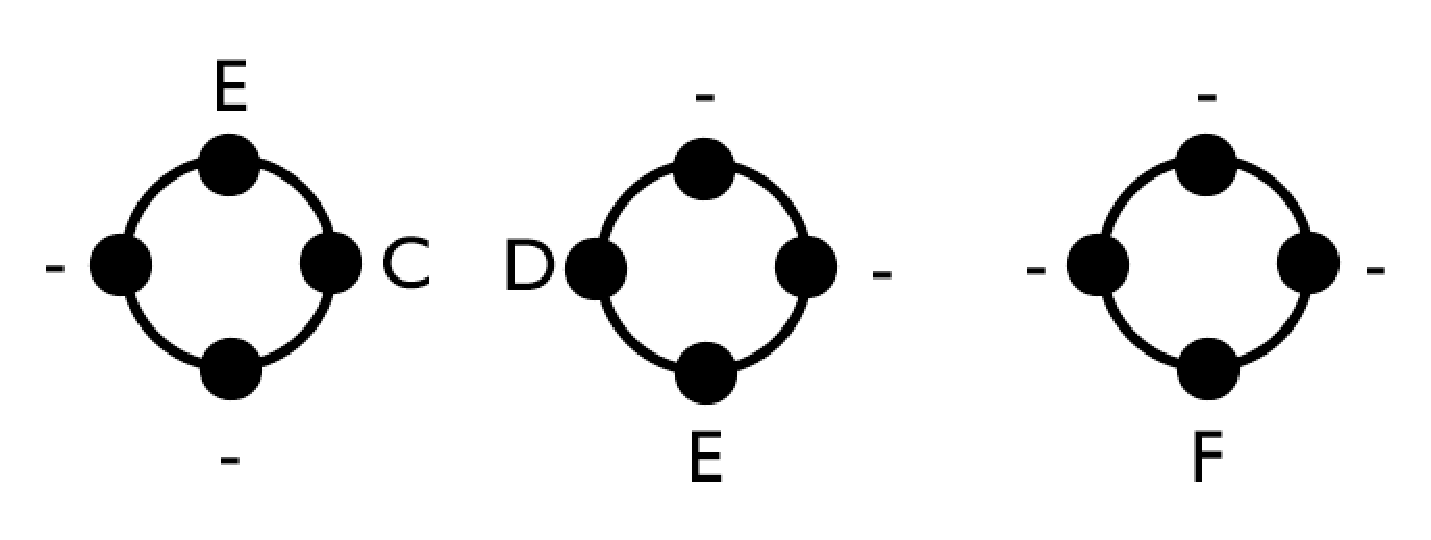
\includegraphics[width=0.4\textwidth]{Figures/ExampleEPS}
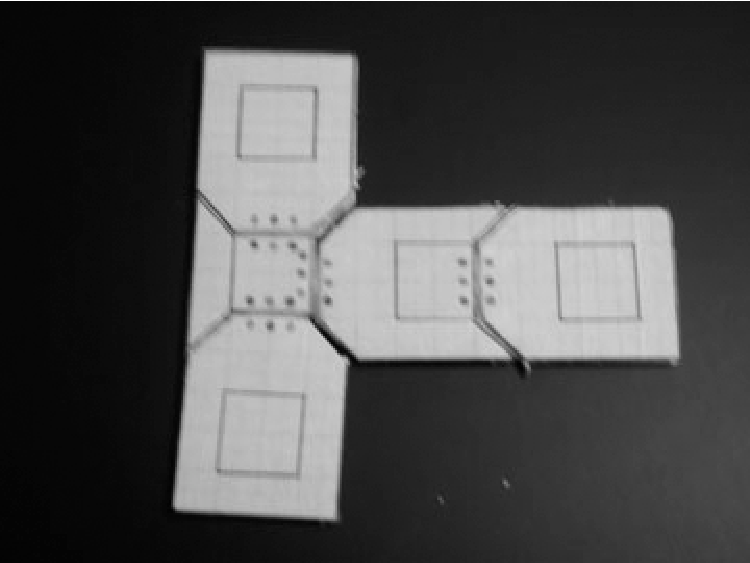
\includegraphics[width=0.4\textwidth]{Figures/PDF-Example}
\end{center}
\caption[ ]{This figure serves as an illustration of how to include a EPS (extended PostScript) graphics file into the document. Note that no extension needs to be specified for any of the graphics files.} 
\label{fig:ExampleEPSandPDF} 
\end{figure}


% MULTI-COLUMN FIGURE

%\begin{figure}
%\begin{center}
%\begin{tabular} {ccc}
%	\includegraphics[width=.3\textwidth]{Figures/PE1-initial.eps} &
%	\includegraphics[width=.3\textwidth]{Figures/PE1-intermediate.eps} &
%	\includegraphics[width=.3\textwidth]{Figures/PE1-final.eps} \\
%	Line: Initial & Line: Intermediate & Line: Final \\
%	\\
%	\includegraphics[width=.3\textwidth]{Figures/PE2-initial.eps} &
%	\includegraphics[width=.3\textwidth]{Figures/PE2-intermediate.eps} &
%	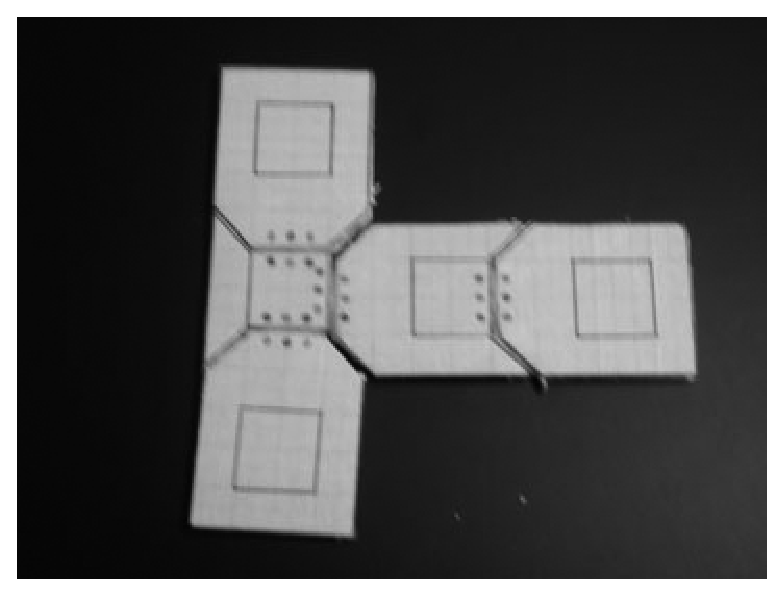
\includegraphics[width=.3\textwidth]{Figures/PE2-final.eps} \\
%	T-shape: Initial & T-shape: Intermediate & T-shape: Final \\
%	\\
%	\includegraphics[width=.3\textwidth]{Figures/PE3-initial.eps} &
%	\includegraphics[width=.3\textwidth]{Figures/PE3-intermediate.eps} &
%	\includegraphics[width=.3\textwidth]{Figures/PE3-final.eps} \\
%	L-shape: Initial & L-shape: Intermediate & L-shape: Final \\
%	\\
%	\includegraphics[width=.3\textwidth]{Figures/PE4-initial.eps} &
%	\includegraphics[width=.3\textwidth]{Figures/PE4-intermediate.eps} &
%	\includegraphics[width=.3\textwidth]{Figures/PE4-final.eps} \\
%	Open Square: Initial & Open Square: Intermediate & Open Square: Final \\
%	\\
%	\includegraphics[width=.3\textwidth]{Figures/PE5-initial.eps} &
%	\includegraphics[width=.3\textwidth]{Figures/PE5-intermediate.eps} &
%	\includegraphics[width=.3\textwidth]{Figures/PE5-final.eps} \\
%	Y-shape: Initial & Y-shape: Intermediate & Y-shape: Final \\
%\end{tabular}
%\end{center}
%\caption[ ]{Results of the five \index{physical} physical systems}
%\label{fig:PhysicalResults}
%\end{figure}


% SIMPLE TABLE

\begin{table}
\caption{\index{physical} Physical encodings}
\vspace{2pt}
\begin{center}
\begin{tabular}{c@{\quad}cc}
\hline
Physical Encoding \# & Shape & Magnetic Encoding \\
\hline\rule{0pt}{12pt}
0	& \index{neutral}Neutral	& (none) \\
\\
1 	& \index{lock}Lock		& 000 \\
2 	& \index{lock}Lock		& 001 \\
3	& \index{lock}Lock		& 010 \\
4	& \index{lock}Lock		& 100 \\
\\
5	& \index{key}Key		& 011 \\
6	& \index{key}Key		& 101 \\
7	& \index{key}Key		& 110 \\
8	& \index{key}Key		& 111 \\
\hline
\end{tabular}
\end{center}
\end{table}



% EXAMPLE OF A COMPLEX TABLE

\begin{table}[htdp]
\caption{System design for the five experiments}
\begin{center}
\begin{tabular}{lll|ll}
	& \multicolumn{2}{c}{{\bf System Design}} 	& \multicolumn{2}{c}{{\bf Desired Entity}} \vspace{0.2cm} \\
	\cline{2-5}
	\multicolumn{1}{l|}{\bf Experiments \hspace{0.5cm}} & 
		\begin{tabular}{c} Component Types \\ (right, top, left, bottom)  \end{tabular} & 
		Rules & 
		\begin{tabular}{c} Number of \\ \index{components} Components \end{tabular} & 
		\begin{tabular}{c|} Symmetric vs. \\ Asymmetric \end{tabular} \\
	\cline{1-5}
	
	\multicolumn{1}{|c}{ Line } & 
	\multicolumn{1}{|p{3cm}}{
		\begin{tabular}{l}
			Type 1: (A, -, A, -) \\  
			Type 2: (B, -, -, -)
		\end{tabular}} & 
	\multicolumn{1}{|p{3cm}}{\begin{tabular}{l}A fits B \\ 
forceX breaks A+B \end{tabular}} & 
	\multicolumn{1}{|c}{ 3 } & 
	\multicolumn{1}{|c|}{\begin{tabular}{c} symmetric \end{tabular}} \\
	\hline
	
	\multicolumn{1}{|c}{ T-shape } & 
	\multicolumn{1}{|p{3cm}}{
		\begin{tabular}{l}
			Type1: (A, -, A, C) \\
			Type2: (-, B, -, -) \\
			Type3: (-, D, -, A)
		\end{tabular}} & 
	\multicolumn{1}{|p{3cm}}{
		\begin{tabular}{l}
			A fits B \\
			C fits D \\
			forceX breaks A+B \\
			forceX breaks C+D 
		\end{tabular}} & 
	\multicolumn{1}{|c}{ 5 } & 
	\multicolumn{1}{|c|}{\begin{tabular}{c} symmetric \\ and \\ asymmetric \end{tabular}} \\
	\hline
	
	\multicolumn{1}{|c}{ L-shape } & 
	\multicolumn{1}{|p{3cm}}{
		\begin{tabular}{l}
			Type1: (A, C, -, -) \\
			Type2: (-, -, B, -) \\ 
			Type3: (-, E, -, D) \\
			Type4: (-, -, -, F)
		\end{tabular}} & 
	\multicolumn{1}{|p{3cm}}{
		\begin{tabular}{l}
			A fits B \\
			C fits D \\
			E fits F \\
			forceX breaks A+B \\
			forceX breaks C+D \\
			forceX breaks E+F 
		\end{tabular}} & 
	\multicolumn{1}{|c}{ 4 } & 
	\multicolumn{1}{|c|}{\begin{tabular}{c} asymmetric \end{tabular}} \\
	\hline
	
	\multicolumn{1}{|c}{ Open Square } & 
	\multicolumn{1}{|p{3cm}}{
		\begin{tabular}{l}
			Type 1: (A, C, -, -) \\
			Type 2: (H, -, B, -) \\
			Type 3: (-, -, B, -) \\
			Type 4: (G, -, -, H)
		\end{tabular}} & 
	\multicolumn{1}{|p{3cm}}{
		\begin{tabular}{l}
			A fits B \\
			C fits D \\
			E fits F \\
			G fits H \\
			forceX breaks A+B \\
			forceX breaks C+D \\
			forceX breaks E+F \\
			forceX breaks G+H
		\end{tabular}} & 
	\multicolumn{1}{|c}{ 8 } & 
	\multicolumn{1}{|c|}{\begin{tabular}{c} symmetric \end{tabular}} \\
	\hline
	
	\multicolumn{1}{|c}{ Y-shape } & 
	\multicolumn{1}{|p{3cm}}{
		\begin{tabular}{l}
			Type 1: (A, -, E, C) \\
			Type 2: (-, D, -, G) \\
			Type 3: (B, -, -, G) \\
			Type 4: (-, -, F, G) \\
			Type 5: (-, -, -, H)
		\end{tabular}} & 
	\multicolumn{1}{|p{3cm}}{
		\begin{tabular}{l}
			A fits B \\
			C fits D \\
			E fits F \\
			G fits H \\
			forceX breaks A+B \\
			forceX breaks C+D \\
			forceX breaks E+F \\
			forceX breaks G+H
		\end{tabular}} & 
	\multicolumn{1}{|c}{ 7 } & 
	\multicolumn{1}{|c|}{\begin{tabular}{c} symmetric \\ and \\ asymmetric \end{tabular}} \\
	\hline
\end{tabular}
\end{center}
\label{default}
\end{table}



% ~~~~~~~~~~~~~~~~~~~~~~~~~~~~~~~~~~~~~~~~~~~~~~~~~~
% CONCLUSIONS
% ~~~~~~~~~~~~~~~~~~~~~~~~~~~~~~~~~~~~~~~~~~~~~~~~~~

\section{Conclusions}
\label{sec:Conclusions}
Here we conclude what we have presented in this research article, which usually consists of a summary of the key findings and a possible outlook on what to do next.


% ~~~~~~~~~~~~~~~~~~~~~~~~~~~~~~~~~~~~~~~~~~~~~~~~~~
% ACKNOWLEDGEMENTS
% ~~~~~~~~~~~~~~~~~~~~~~~~~~~~~~~~~~~~~~~~~~~~~~~~~~

\section*{Acknowledgements}
Financial support for this research is provided by NSERC, the Natural Sciences and Engineering Research Council of Canada.




% ~~~~~~~~~~~~~~~~~~~~~~~~~~~~~~~~~~~~~~~~~~~~~~~~~~
% References: Bibliography
% ~~~~~~~~~~~~~~~~~~~~~~~~~~~~~~~~~~~~~~~~~~~~~~~~~~

\bibliographystyle{splncs}
\bibliography{References} % add bibliography file here


% ~~~~~~~~~~~~~~~~~~~~~~~~~~~~~~~~~~~~~~~~~~~~~~~~~~
% Index (optional): collects items in text from \index{...} command
% ~~~~~~~~~~~~~~~~~~~~~~~~~~~~~~~~~~~~~~~~~~~~~~~~~~
%\printindex

\end{document}
